\documentclass[a4page]{article}
\usepackage[14pt]{extsizes} % для того чтобы задать нестандартный 14-ый размер шрифта
\usepackage[utf8]{inputenc}
\usepackage[russian]{babel} % поддержка русского языка
\usepackage{amsmath}  %  математические символы
\usepackage[left=20mm, top=15mm, right=15mm, bottom=30mm, footskip=15mm]{geometry} % настройки полей документа
\usepackage{indentfirst} % по умалчанию убирается отступ у первого абзаца в секции, это отменяет это.
\usepackage{paralist} % добавить компактные списки (compactitem, compactenum, compactdesc)
\usepackage{microtype}
\usepackage{fancyvrb}
\usepackage{framed}
\usepackage{url}


\usepackage{float}
\floatstyle{ruled}

\usepackage{graphicx}
\usepackage{csquotes}

\usepackage[
    backend=biber, 
    sorting=nyt,
    bibstyle=gost-numeric,
    citestyle=gost-numeric
]{biblatex}

\usepackage[
bookmarks=true, colorlinks=true, unicode=true,
urlcolor=black,linkcolor=black, anchorcolor=black,
citecolor=black, menucolor=black, filecolor=black,
]{hyperref}

\addbibresource{sources.bib}

\renewcommand{\baselinestretch}{1.35}

%\usepackage{minted}

\begin{document} % начало документа
 
 
% НАЧАЛО ТИТУЛЬНОГО ЛИСТА
\begin{titlepage}

\begin{center}
\hfill \break
\textbf{
\large{РОССИЙСКИЙ УНИВЕРСИТЕТ ДРУЖБЫ НАРОДОВ}\\
\normalsize{Факультет физико-математических и естественных наук}\\ 
\normalsize{Кафедра прикладной информатики и теории вероятностей}\\
}
\vspace*{\fill}
\Large{\textbf{ДОКЛАД\\ на тему <<Преобразование аналоговых сигналов в цифровые и обратно: АЦП и ЦАП>>}}
\\
\underline{\textit{\normalsize{Дисциплина: Сетевые технологии}}}
\vspace*{\fill}

\end{center}
 
 \begin{flushright}
 Студент: \underline{Генералов Даниил}\\ \vspace{0.5cm}
 Группа: \underline{НПИбд-01-21}
 \end{flushright}
 
 
\begin{center} \textbf{МОСКВА} \\ 2023 г. \end{center}
\thispagestyle{empty} % выключаем отображение номера для этой страницы
 
\end{titlepage}
 % КОНЕЦ ТИТУЛЬНОГО ЛИСТА

\newpage

\tableofcontents

\newpage

\newcommand{\code}[1]{\texttt{#1}}

\section{Введение}

Наши компьютеры работают на электричестве.
Для того, чтобы компьютер работал надежно, мы решили, что на каждом проводе электричество будет иметь только два состояния:
либо оно есть, либо его нет.

Но электричество имеет другие варианты -- оно может присутствовать, но не сильно.
В некоторых ситуациях компьютеру важно знать про эти промежуточные состояния.
Для того, чтобы преобразовывать между миром цифровых сигналов и миром аналоговых сигналов,
существуют устройства: Аналогово-\-Цифровые Преобразователи и Цифрово-\-Аналоговые Преобразователи.

\subsection{Применения аналоговых сигналов}

Когда мы передаем или получаем сигнал по проводу, нам важно напряжение на этом проводе.
Напряжение -- это разность потенциала между этим проводом и каким-то общим проводником, который по определению имеет напряжение $0V$.

По законам электромагнетизма, проводники с током создают вокруг себя магнитное поле, а изменение магнитного поля приводит к изменению тока в проводниках -- 
что подразумевает изменение потенциала этого проводника.
Другими словами, изменяющийся ток рядом с проводом вызывает помехи, которые меняют напряжение на проводе.

Это весьма проблематично для компьютеров:
внутри них постоянно происходят изменения тока при переключении транзисторов,
а они также находятся в близости от очень крупного магнитного поля, которое меняется 50 раз в секунду и вызвано 240-вольтной электрической проводкой в стенах зданий.

Для того, чтобы компьютер не был подвержен этим помехам, было решено ограничить набор напряжений, которые могут появляться в его схемах.
Допустим, микросхема, которая отправляет сигнал, будет ставить свои выводы либо на значение $5V$, либо $0V$.
Помехи на этом проводе будут не слишком большими -- например не больше $\pm 0.5V$.
Теперь, если получающая микросхема будет воспринимать любое напряжение больше $3.5V$ как высокое,
а любое напряжение меньше $1.5V$ как низкое,
то она всегда будет интерпретировать входящий сигнал в точности как он был отправлен.
Так работают цифровые схемы, которые являются основой всех современных компьютеров.


В каких же ситуациях компьютеру может быть важно знать про промежуточные состояния напряжений?
Вкратце, в любой ситуации, когда нужно взаимодействовать с какой-то внешней системой, которая по своей сути является аналоговой --
а таких вокруг компьютеров сегодня довольно много. 

Например, радио-волны -- это сугубо аналоговый феномен. Для того, чтобы принимать радио-волны -- даже такие, которые кодируют цифровой сигнал -- 
нужна схема, которая будет извлекать из радио-волны эти цифровые данные -- в определенном смысле это и есть аналогово-цифровой преобразователь.
Более того, радио-связь становится все более важной, и уже существует много протоколов радио-связи,
все из которых тяжело реализовать в микросхемах внутри одного смартфона;
поэтому сейчас становятся все популярнее так называемые SDR, \emph{software-defined radio},
которые по сути являются специализированным высокоскоростным процессором, подключенным к цифрово-аналоговому преобразователю,
который выдает сигналы, которые модулируются и непосредственно отправляются на антенну для передачи.

Говоря о смартфонах, им важно знать, где происходит нажатие на их сенсорный экран.
Для этого под стеклом этого экрана находится сетка тонких проводников, к которым применяется напряжение
Прибли\-жающийся к ним палец образует кон\-ден\-сатор, который изменяет напряжение на этих проводах.
Затем аналогово-\-цифровые пре\-образо\-ватели позволяют считать это напряжение,
и в том месте, где оно сильно отличается от стандартного,
должен находится палец, который только что нажал на кнопку.

Эта кнопка была изображена на жидко-кристаллическом экране непосредственно под сенсорной панелью.
ЖК-экраны имеют источник света, который постоянно светит белым светом,
и перед ним находится фильтр, который затемняет его в нужных местах,
чтобы образовать изображение.
Этот фильтр состоит из отдельных ячеек, или пикселей,
которые становятся более или менее яркими в зависимости от уровня напряжения на них.
Для того, чтобы пиксели могли иметь промежуточные уровни яркости,
а не только быть включенными или выключенными,
требуется цифрово-аналоговый преобразователь, чтобы создать этот промежуточный уровень напряжения.

Возможно, самое известное применение АЦП и ЦАП в компьютерах -- это аудиоустройства.
Звук попадает на микрофон, который создает переменное напряжение,
которое с помощью АЦП записывается в компьютер,
а затем с помощью ЦАП преобразуется в копию исходного сигнала,
который затем можно передать в усилитель и на динамик,
чтобы воспроизвести тот же самый звук.

Наконец, одно из менее очевидных применений аналоговых сигналов -- это при взаимодействии с физическими объектами.
В различной робототехнике часто нужно измерить аналоговые значения, которые связаны с физическим состоянием робота:
например, ориентацию компаса, угол отклонения какого-то соединения, или уровень давления в газовой ёмкости.
Аналогично, иногда нужно создавать аналоговые сигналы на выходе:
например, чтобы мотор не был полностью включен, а только наполовину.
Хотя для некоторых таких задач существуют сенсоры и актуаторы, по своей природе являющиеся чисто цифровыми,
также иожно найти множество таких, которые нет;
для таких устройств потребуется преобразование между аналог\-овым миром, где живет само устройство,
и цифровым миром кон\-троллеров.


\section{Дизайн схем преобразователей}

Для того, чтобы решать все эти задачи, нужно сначала построить АЦП и ЦАП, которые позволят переходить между аналоговыми и цифровыми сигналами.
Есть несколько разных способов делать это.

\subsection{ЦАП}
Более простая из двух операций -- превращение цифрового сигнала в аналоговый.

Один из простых способов сделать это -- \emph{широтно-импульсный модулятор}.
Схема создает импульсы, ширина которых меняется в зависимости от мгновенного значения,
и эти импульсы затем передаются в частотный фильтр.
Частые, но короткие импульсы таким образом превращаются в постоянное, низкое напряжение,
а частые и длинные импульсы -- в постоянное, высокое напряжение.
Эти импульсы можно создать с помощью всего лишь одного вывода на микроконтроллере,
что позволяет сконструировать сигнал с меняющейся шириной импульса с помощью таймеров микроконтроллера.

Для других дизайнов ЦАП требуется передать мгновенное значение на какого-то вида шину.
Например, бинарно-взвешенный ЦАП состоит из набора резисторов,
где каждый следующий резистор имеет сопротивление в два раза меньше.
Затем, старший бит отвечает за то, подключен ли в цепь самый большой резистор,
следующий бит -- за то, подключен ли резистор поменьше, и так далее.
Итоговая комбинация резисторов подключается к константному резистору, создавая делитель напряжения,
и значение напряжения в точке деления находится где-то между максимальным и нулем.
Для $n$-битного ЦАП, который использует такой подход,
требуется $n$ резисторов.

Однако, если какие-то из этих резисторов имеют неточные значения,
то их комбинация будет иметь пропорционально меньшую точность.
Для самых требова\-тельных применений можно взять больше резисторов -- а именно $2^n-1$.
Они будут создавать точное выходное напряжение для каждого возможного значения ЦАП,
и входящее значение лишь переключает, какой конкретно из этих выходов сейчас подключен.
Это количество очень быстро растет -- для 8-битного ЦАП нужно 255 точных резисторов,
а для 16-битного уже 65535 -- но этот дизайн самый быстрый и самый точный.
Также, эти резисторы изо\-лированы друг от друга, поэтому любая произ\-водственная неточность
не приводит к каскаду ошибки:
вместо этого они влияют только на это одно возможное значение,
и тем самым становятся частью фонового уровня шума.

\subsection{АЦП}
Преобразование из аналогового сигнала в цифровой -- сравнительно более сложная операция.
Фундаментальным компонентом для этого выступает \emph{компаратор} -- специальная версия операционного усилителя,
которая принимает два сигнала, $V_{+}$ и $V_{-}$,  и выдает высокое напряжение когда $V_{+}>V_{-}$ и низкое иначе.

Компараторы требуют довольно высокое количество транзисторов, поэтому многие дизайны пытаются минимизировать их количество.
Например, один дизайн использует только один компаратор, таймер и генератор пило-образной волны -- сигнала, который постепенно повышает напряжение,
а затем быстро возвращается к нулю.
Когда волна имеет нулевое значение, таймер обнуляется,
а когда волна пересекает значение сигнала, таймер считывается и сохраняется.
Эту волну можно создать с помощью схемы-интегратора,
но тогда она будет подвержена изменениям частоты при изменениях температуры;
вместо этого ее часто генерируют с помощью цифрового счетчика и ЦАП --
то есть, чтобы сделать АЦП, нужно иметь ЦАП.
У этого дизайна АЦП есть еще примущество: чтобы добавить дополнительные каналы, нужно добавить только еще один регистр счётчика и компаратор;
генератор волны можно использовать несколько раз.

\begin{figure}
    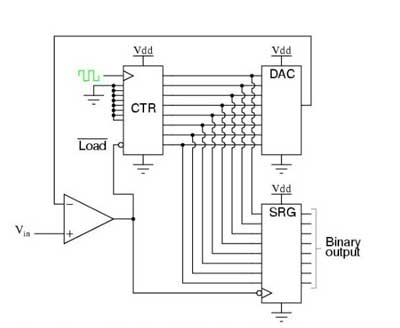
\includegraphics[width=\linewidth]{ramp-adc.jpg}
    \caption{Схема АЦП с пило-образным генератором~\cite{web:polytechnic-adc}}
    \label{fig:ramp-adc}
  \end{figure}


  Идея использовать ЦАП, чтобы реализовать АЦП, появляется в нескольких других дизайнах.
  Например, один дизайн использует ЦАП, регистр и один компаратор, чтобы выполнить бинарный поиск по напряжениям.
  Сначала создается напряжение 50\%, и входной сигнал сравнивается с ним.
  Если входной сигнал выше этого, то мы запоминаем, что старший бит должен быть задан,
  если меньше -- что должен быть очищен.
  После этого мы тестируем последующие биты,
  и последний из битов тестируем дважды.
  Это дает нам значение, которое нужно передать ЦАП, чтобы получить лучшее возможное приближение входного сигнала к АЦП,
  которое затем можно вывести.


  Оба из этих дизайнов требуют несколько тактов, чтобы зафиксировать значение,
  и это потому что они должны использовать один компаратор несколько раз в разных конфигурациях, чтобы найти точное значение сигнала.
  Если же использовать $2^n$ компараторов одновременно, то можно сравнить один и тот же сигнал с несколькими расчетными напряжениями,
  и тем самым за один такт найти нужное напряжение.
  Поэтому именно эта схема используется в самых высокоскоростных примененях, вроде радаров, радио-приемников и считывателей жестких дисков.
  Ещё одно из преимуществ такой схемы -- изменив резисторы, можно получить нели\-нейное считывание сигнала, что может быть полезно для сигналов,
  чьё значение не равномерно распределено по времени.


  \begin{figure}
    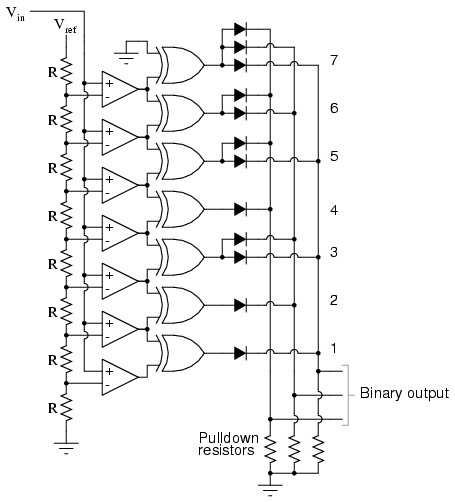
\includegraphics[width=\linewidth]{flash-adc.png}
    \caption{Схема Flash ADC~\cite{web:digitalCircuitsAdc}}
    \label{fig:flash-adc}
  \end{figure}

  Из-за того, что эта схема имеет преимущества в точности, но также значительно дороже в производстве,
  часто в практических задачах используют каскад из нескольких типов АЦП.
  Сначала более дешевый, но менее точный АЦП считывает приблизительное значение сигнала.
  Затем, это значение передается в ЦАП, а затем с помощью операционного усилителя вычитается из исходного сигнала.
  Получившийся сигнал представляет собой низкоуровневый точный сигнал,
  который затем можно проанализировать этим более точным типом АЦП,
  а затем поставить его вывод в менее значимые биты финального значения измеренного сигнала.


\section{Теория аналогово-цифрового кодирования}

Стандартный способ представления волновых данных в компьютере -- \emph{импульсно-кодовая модуляция} (pulse-code modulation, PCM).
Аналоговый сигнал представляется как набор измерений (\emph{samples}), которые были взяты у сигнала в равномерно-распределенные моменты времени.
Эти измерения производятся с помощью АЦП.

\begin{figure}
  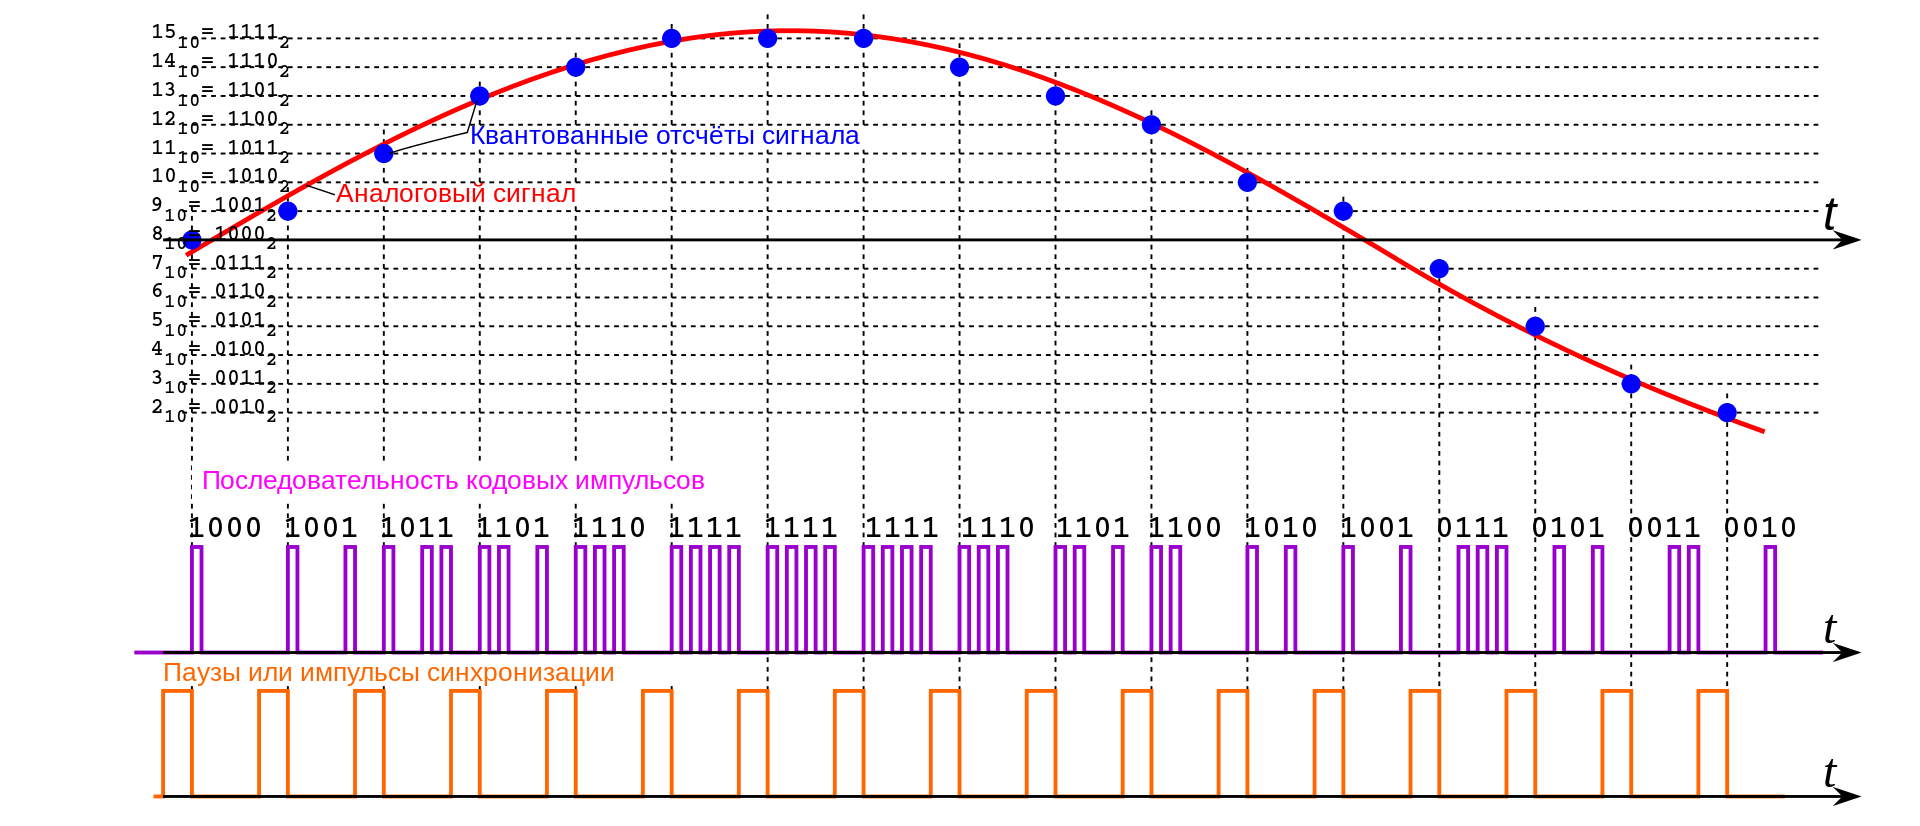
\includegraphics[width=\linewidth]{Pcm-ru.svg.png}
  \caption{Пример оцифровки сигнала~\cite{wiki:pcm}}
  \label{fig:pcm-wave}
\end{figure}

Фактически, волна преобразуется в набор точек.
По горизонтали эти точки распределены равномерно, и находятся на одинаковом расстоянии друг от друга.
По вертикали точки могут принимать одно из ограниченного количества позиций, которые определяются количеством битов у АЦП.

Процесс преобразования постоянного во времени сигнала в разорванный по точкам (дискретный) сигнал называется \emph{дискретизацией}.
Количество точек, которые записываются горизонтально в течении одной секунды, называется \emph{частотой дискретизации},
а количество разных вертикальных значений -- количество \emph{уровней квантизации} -- определяется количеством битов АЦП.

\begin{figure}
  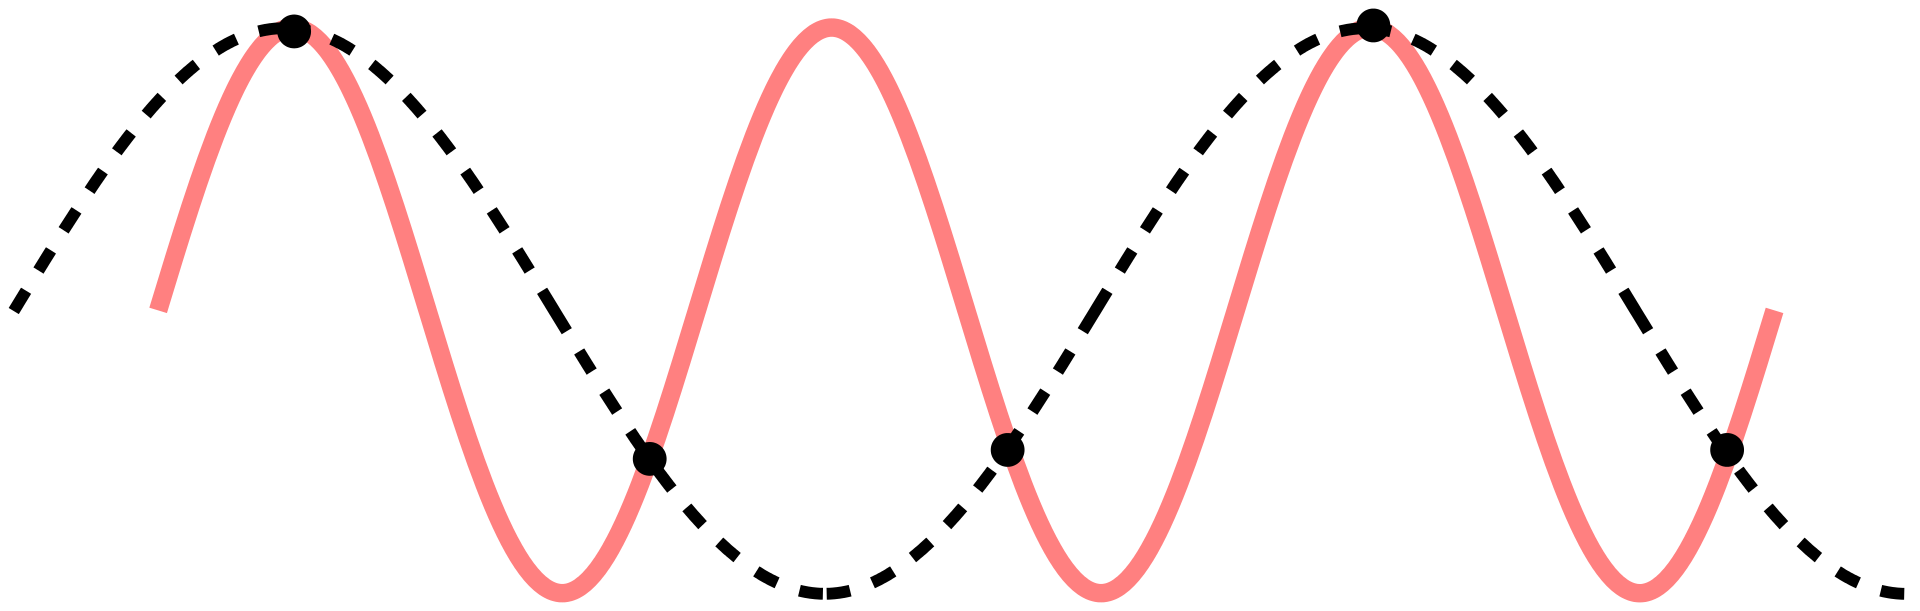
\includegraphics[width=\linewidth]{CPT-sound-nyquist-thereom-1.5percycle.svg.png}
  \caption{Пример недостаточной частоты дискретизации. Красная волна имеет частоту в 1.5 раза выше частоты дискретизации, и поэтому измерения -- черные точки -- образуют пунктирную волну более низкой частоты~\cite{enwiki:1174270402}}
  \label{fig:pcm-samples}
\end{figure}

Если задать частоту дискретизации слишком низкой, то высокочастотные компоненты сигнала будут невозможно представить в записи.
Например, на рисунке~\ref{fig:pcm-samples} показано, как недостаточная частота дискретизации приводит к тому,
что высокочастотный сигнал записывается как низкочастотный сигнал.

Чтобы выбрать правильную частоту дискретизации, следует использовать теорему отсчетов,
также известную как теорему Котельникова, Найквиста и/или Шеннона~\cite{enwiki:1174270402}.
Согласно этой теореме, можно с точностью представить дискретизированные сигналы,
частота которых ниже половины частоты дискретизации.
Например, человеческий голос имеет основные частоты в диапазоне от 300Гц до 3400Гц~\cite{web:fs-voice-band},
и поэтому телефонные системы используют частоту дискретизации 8000Гц.
Аналогично, общий диапазон частот, которые слышит человек, обычно не выше 20кГц,
поэтому музыка на компакт-дисках имеет частоту дискретизации выше 40кГц.

Количество уровней квантизации также влияет на точность воспроизведения сигнала.
Однако здесь это свойство влияет на уровень шума:
чем меньше уровней квантизации, тем выше порог шума сигнала,
и тем меньше динамический диапазон, который можно представить в сигнале.
Это можно наглядно увидеть в изображениях,
где, чем меньше количество битов на пиксель,
тем меньше точных деталей можно увидеть,
потому что похожие цвета превращаются в одинаковые.
Также, динамический диапазон становится более ограниченным --
как можно увидеть на рисунке~\ref{fig:downsampled-image},
в низкоцветных версиях изображений меньше разницы между самыми яркими и самыми тусклыми частями изображения.


\begin{figure}
  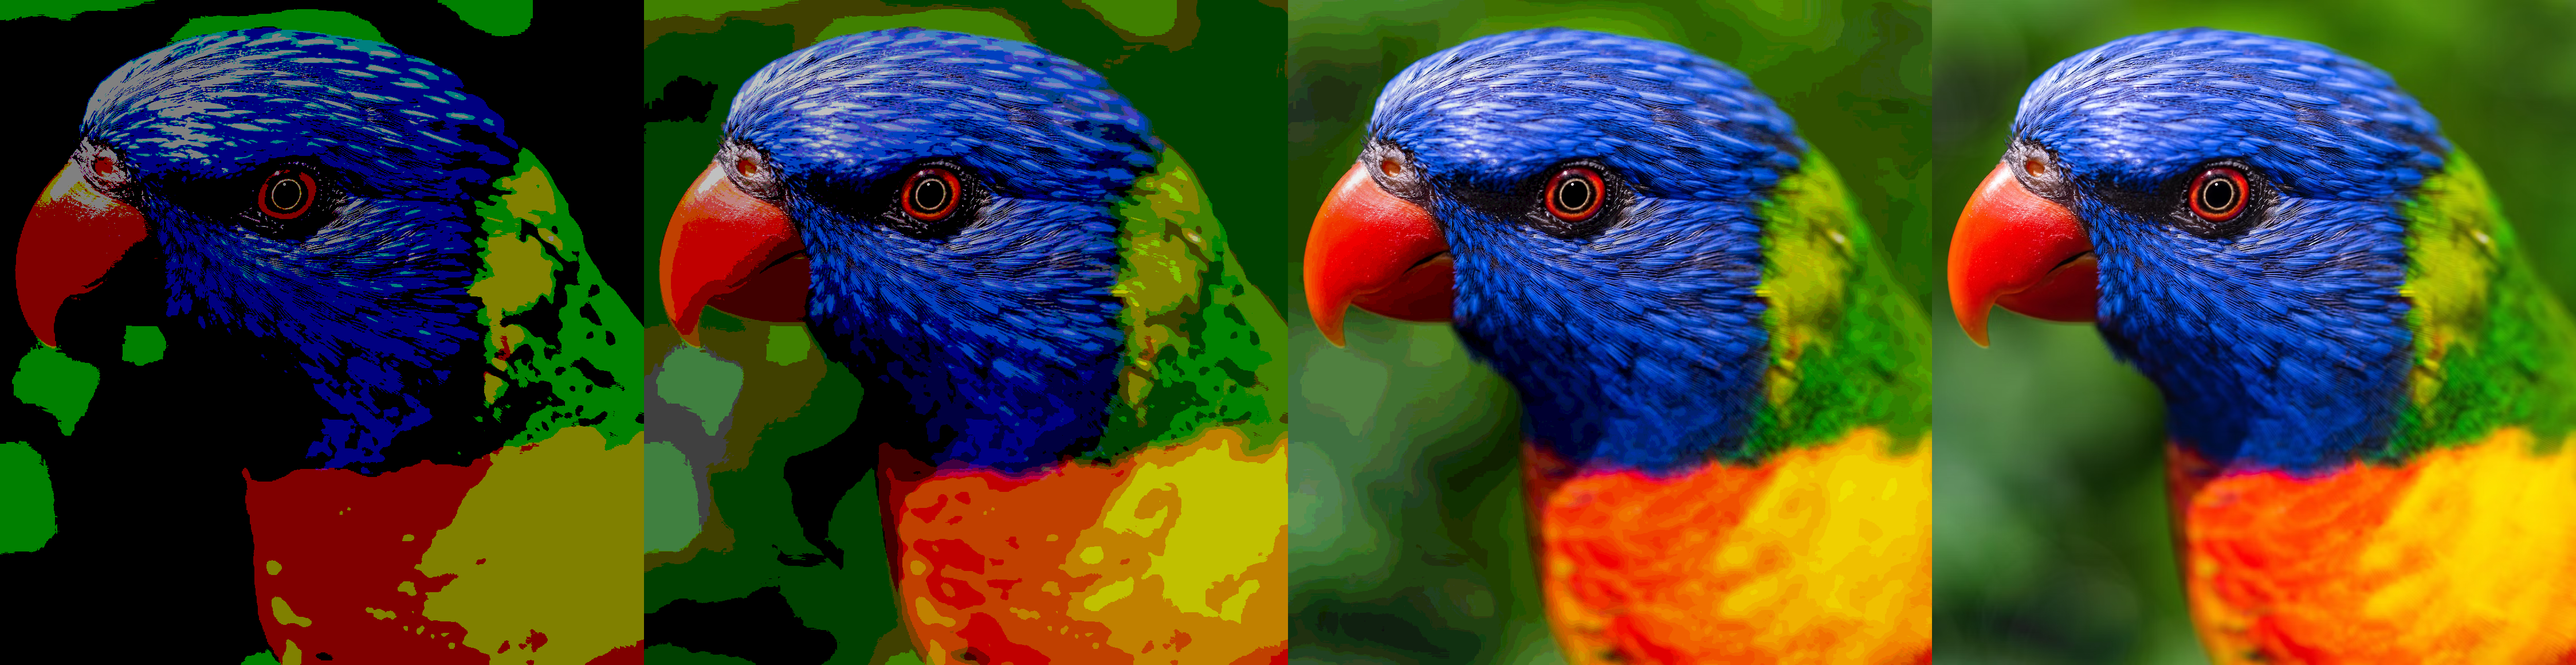
\includegraphics[width=\linewidth]{chicken-colorized.png}
  \caption{Пример уровней дискретизации. Справа -- изначальное изображение, слева -- версии этого изображения, дискретизированные до 1, 2 и 4 битов на пиксель}
  \label{fig:downsampled-image}
\end{figure}

\section{Использование волновых данных}

После того, как сигнал был считан с помощью АЦП, с ним нужно что-то сделать.
В самом простом случае можно получить обратно тот же самый сигнал,
но это весьма бесполезно делать сразу же;
гораздо полезнее воспроизвести сигнал в каком-то далеком месте или в какое-то далекое время.
Однако, и передача, и хранение PCM-данных осложняется тем, что объем данных очень высок.

Например, аудио на компакт-диске имеет два канала, каждый из которых представлен 16-битными samples, которых происходит 44100 в секунду.
Это значит, что в секунду проходит 1411200 бит, или 172.2 кбайт; за минуту пройдет больше 10Мбайт.
В то время, когда стандарт CD был утвержден, почти не существовало форматов, которые могли бы хранить такое количество информации:
даже дискеты высокой плотности, которые хранят 1.44Мбайт, смогут сохранить только 8.5 секунд аудио в таком качестве.
Ещё более сложно передавать эти данные: в идеальных условиях, телефонная линия может передавать 56кбит/с, а этот аудио-сигнал требует ширину канала в 24 раза больше.

Чтобы обойти эти ограничения, можно снизить качество сигнала, понизив частоту дискретизации и/или количество уровней квантизации.
Также можно использовать схемы сжатия, которые бывают с потерями и без потерь.
Сжатие без потерь оставляет сигнал идентичным, обменивая ширину канала на сложность интерпретации этого сигнала.
Один из самых простой способ сжатия -- дельта-кодирование -- использует тот факт, что в большинстве волн амплитуда меняется плавно,
и поэтому сохраняется разность между предыдущим и следующим sample, и меньшие абсолютные значения разности имеют меньшую длину символа.
Такое кодирование сохраняет форму волны с точностью, но требует дополнительных вычислений для извлечения этой волны.

Сжатие с потерями позволяет достичь гораздо большей экономии объема, но требуют весьма сложных и нетривиальных вычислений,
а также снижают качество сигнала.
Эти алгоритмы настраиваются, чтобы сохранять те спектральные характеристики сигнала,
которые больше всего влияют на восприятие этого сигнала;
например, MP3-кодирование основано на разложении аудио-сигнала в чистые синусоиды, а затем подавлении наименее значимых из них
(похоже на DCT, \emph{discrete cosine transform}, в кодировании JPG),
но он также тщательно настраивался, чтобы слушатели не услышали разницы на примерах определенных песен~\cite{web:mp3-ghost}.

Существует много различных алгоритмов сжатия волновых данных с потерями,
и большинство из них предназначены для аудио:
те научные задачи, которые работают с волновыми данными,
чаще всего записывают сигнал без сжатия или с сжатием без потерь.

Алгоритмы для сжатия аудио различаются по своим специализациям,
которые определяют их эффективность и точность в сжатии различных типов сигналов.
На рисунке~\ref{fig:opus-spectro} приведено сравнение спектрограмм некоторых алгоритмов,
которые все теоретически предназначены для кодирования музыки,
но могут быть настроены, чтобы экономить память в обмен на ограничение воспроизводимого диапазона --
что весьма важно при передаче человеческого голоса по линиям цифровой коммуникации.

\begin{figure}
  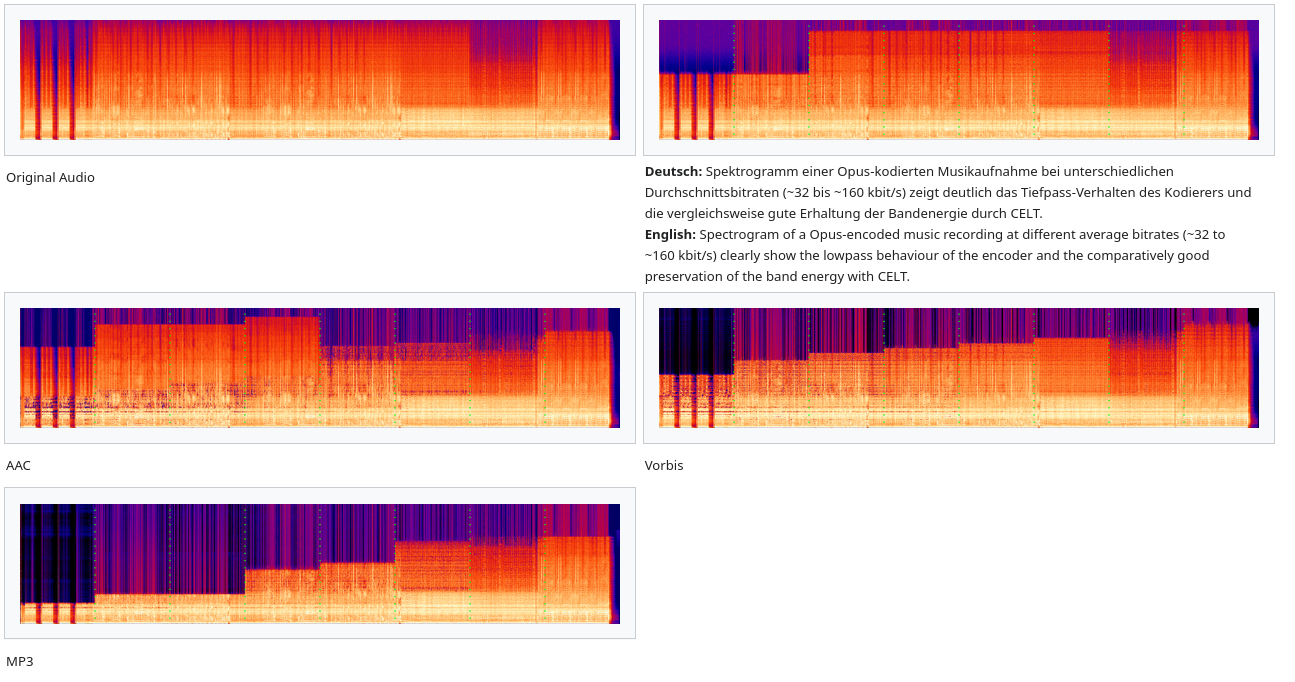
\includegraphics[width=\linewidth]{opus-comparison.png}
  \caption{Пример спектрограмм аудио-файла, который был сжат алгоритмами Opus, AAC, Vorbis и MP3~\cite{wiki:opus-spectro}}
  \label{fig:opus-spectro}
\end{figure}

\subsection{Как CD-аудио связано с телевизором}

Многие современные аудио-приложения работают с частотой дискретизации в 44100Гц --
довольно неочевидная частота.
Чтобы понять, почему именно эта частота стала стандартной,
нужно вернуться к зарождению цифрового аудио.

Как уже упомянуто, цифровое аудио требует очень большого объема данных,
и сначала почти не было форматов, которые могут хранить такое количество данных.
Однако в 1980-х было найдено решение, которое уже давно существовало на рынке:
самый широкополосный сигнал, который было нужно записывать до этого времени -- это телевизионный сигнал в видеомагнитофоне.

Было изобретено устройство -- так называемый PCM-адаптер -- которое принимало на вход аналоговый аудио-сигнал,
оцифровывало его, а затем выдавало телевизионный видео-сигнал,
который содержал импульсы, которые кодировали этот аудио-сигнал,
а также информацию для коррекции ошибок. Один кадр из такой системы кодирования показан на рисунке~\ref{fig:pcm-adapter-vid}.


\begin{figure}
  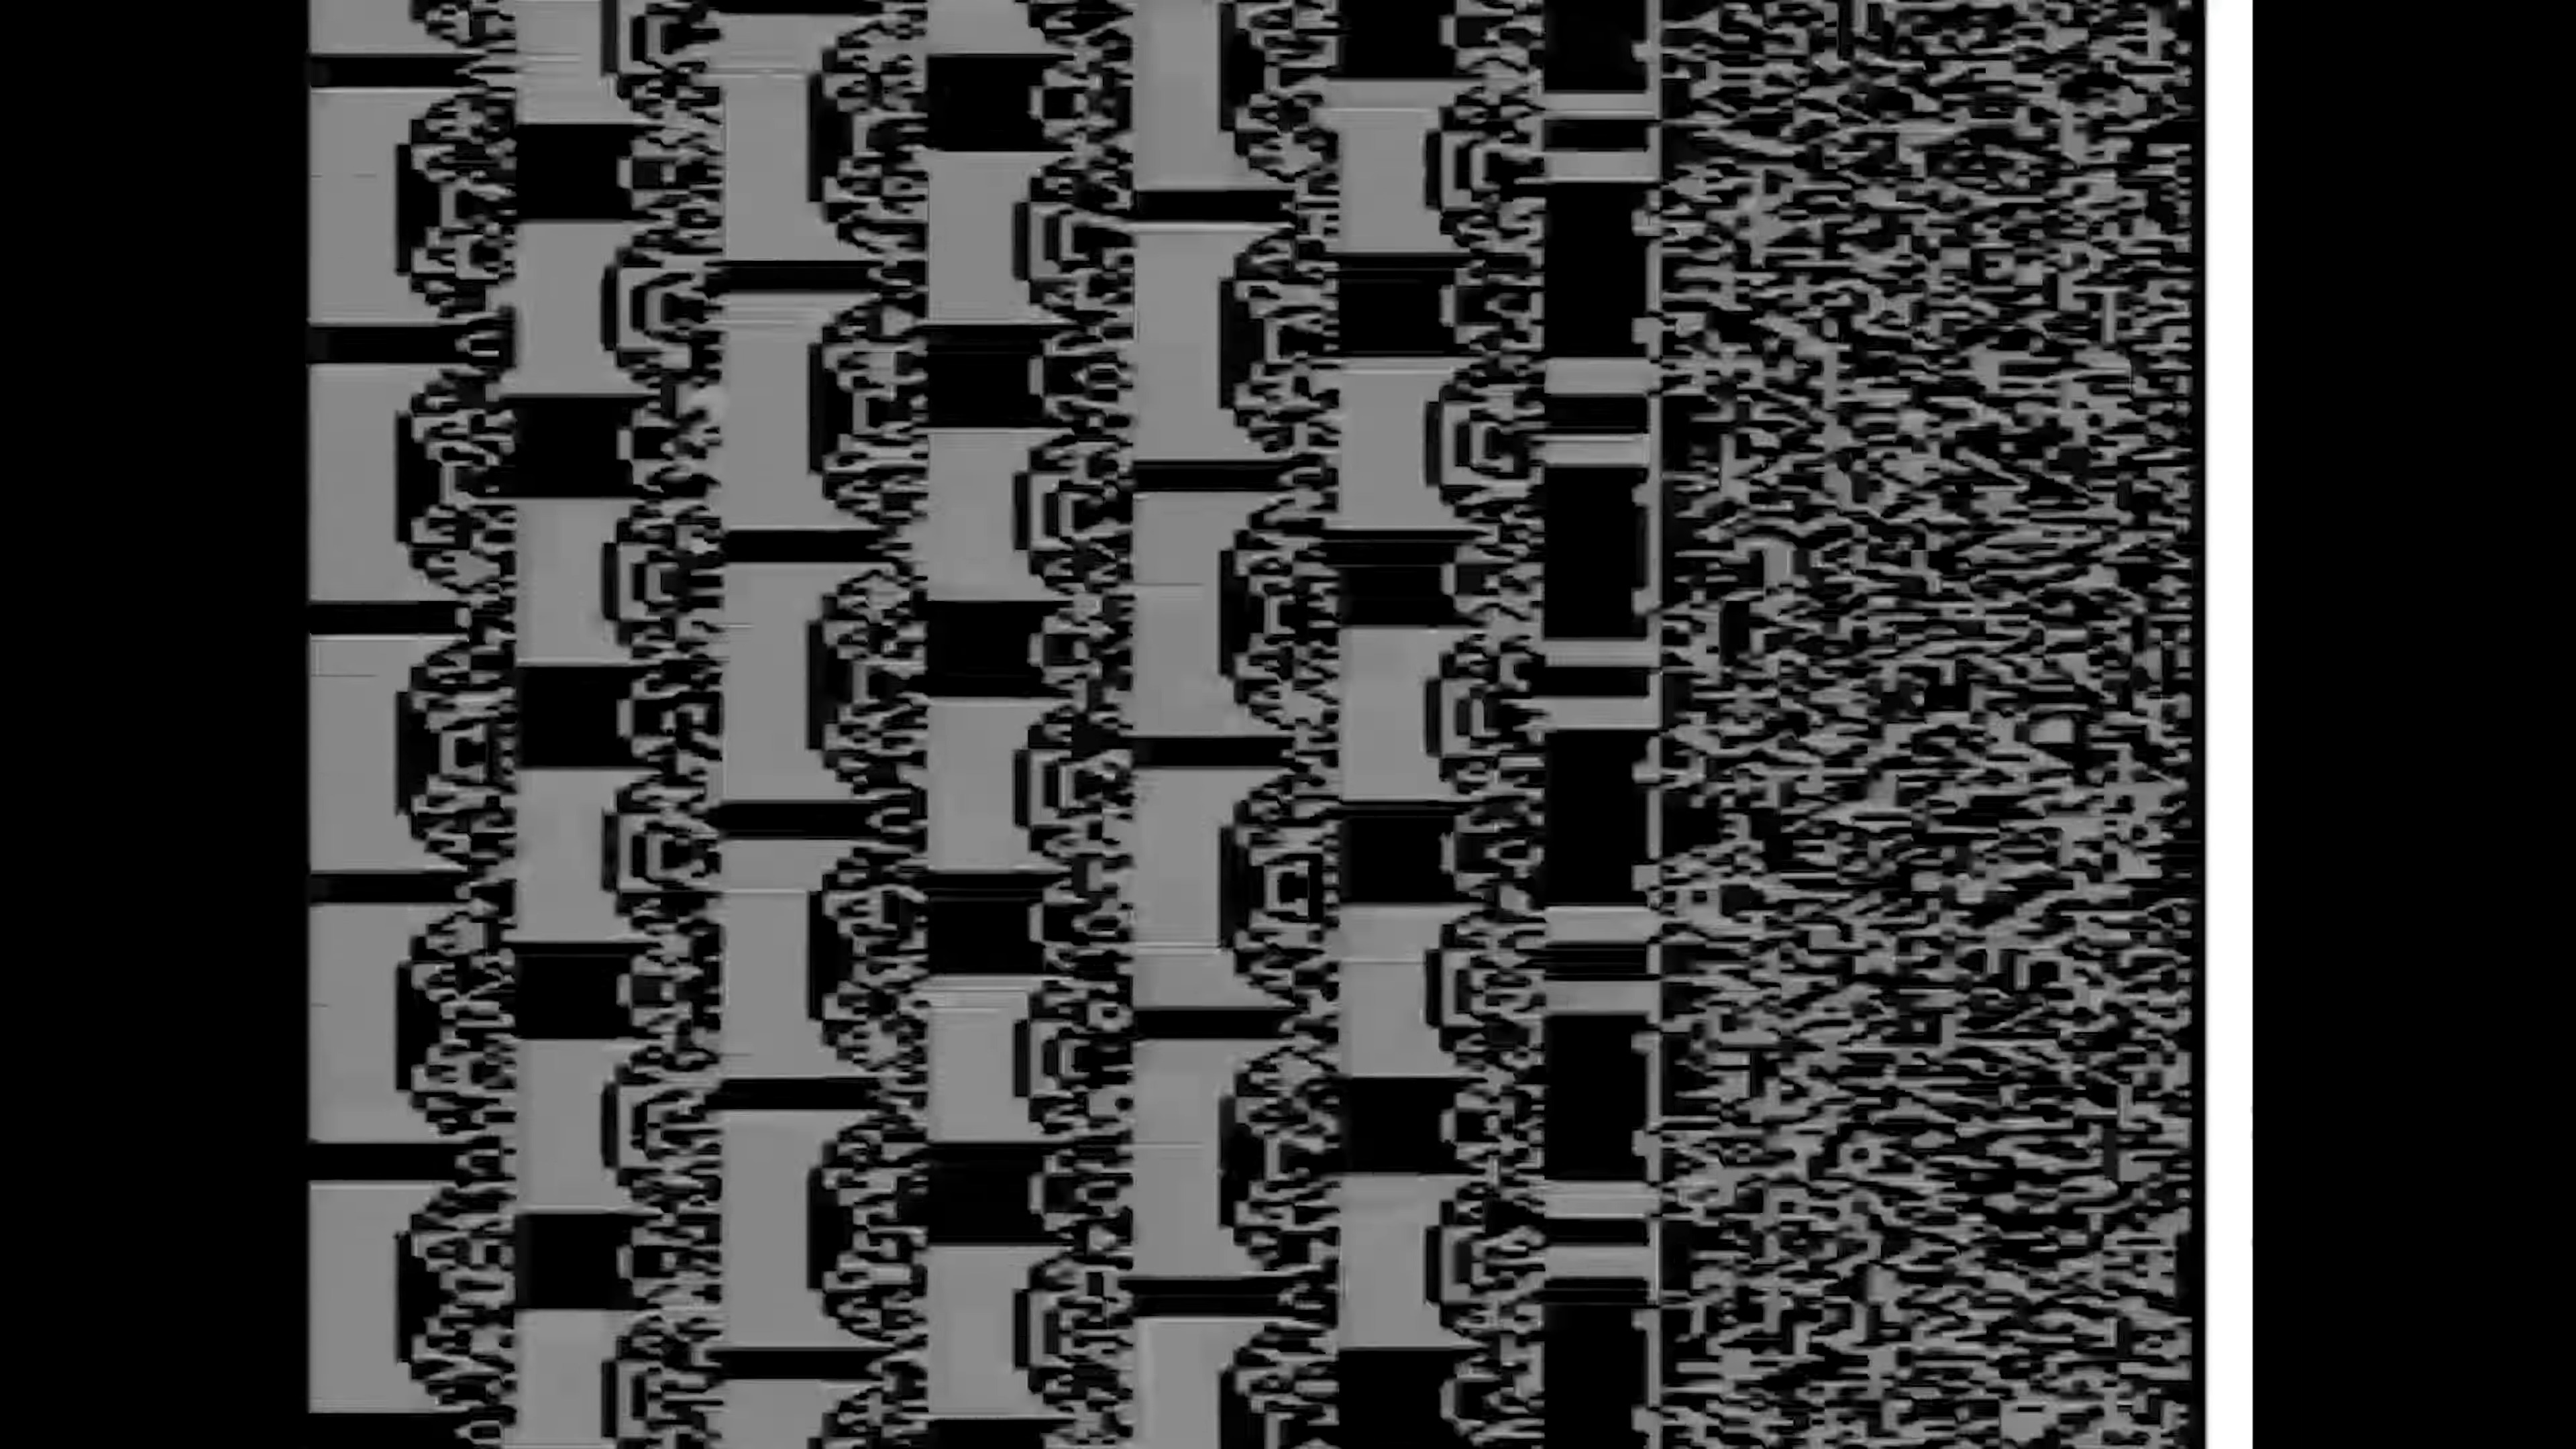
\includegraphics[width=\linewidth]{pcm-adapter-frame.jpg}
  \caption{Кадр, снятый с PCM-адаптера, который получает на вход синусоиду~\cite{web:pcm-adapter-vid}}
  \label{fig:pcm-adapter-vid}
\end{figure}

Этот формат должен быть совместим с телевизионным сигналом,
который состоит из где-то около 15000 горизонтальных линий в секунду,
хотя некоторые из этих линий нельзя использовать, потому что они составляют часть пространства между двумя кадрами.
Чтобы частота дискретизации была больше 40кГц, нужно, чтобы на одной горизонтальной линии было больше одного sample;
достаточно, чтобы их было три, или шесть для стерео-сигнала.
Каждый из них имел 16 битов -- количество уровней квантизации было равно 

Более точно, мы говорим о двух стандартах видео-сигнала -- PAL, который используется в Европе,
и NTSC, который используется в США.
В PAL частота видео-полей равна 50Гц, и каждый кадр состоит из двух полей, в каждом из которых можно использовать 294 линии;
в NTSC же частота полей -- 60Гц, и в каждом поле можно использовать 245 строки.

Поскольку этот стандарт должен быть совместим и с PAL, и с NTSC,
то используемая частота должна делиться на 50 и на 60, а на каждой строке три значения.
Следовательно, используемая частота должна быть кратной  900Гц,
а также быть больше 40кГц, но меньше 46.875кГц.
Внутри этого диапазона самая высокая допустимая частота -- 44.1кГц.

Следует заметить, что для PCM-адаптеров, предназначенных для использования в видеомагнитофонах потребительского класса в NTSC,
частота дискретизации на 0.1\% ниже и равняется 44056Гц.
Это связано с тем, что такие видеомагнитофоны записывают цветное телевидение,
а в стандарте NTSC, из-за интересных причин обратной совместимости,
цветное телевидение имеет частоту кадров не 30Гц, а 29.97Гц -- ровно на 0.1\% ниже.

Когда разрабатывался стандарт CD-аудио, существовал только этот способ записи цифрового аудио.
Чтобы звук оказался на диске, он должен был быть как-то записан,
и в те времена он был бы записан на видеокассету и имел бы частоту дискретизации 44100Гц,
и это была бы стерео-запись с глубиной квантизации 16 битов.
Поэтому было принято решение использовать именно эти параметры,
и они были превращены из фактического стандарта PCM-адаптеров
в настоящий стандарт CD-аудио.
После этого, когда возникла потребность работать с цифровым аудио на компьютере,
форматы файлов должны быть совместимыми с CD-аудио,
а также с более новыми изобретениями вроде Digital Audio Tape,
которая использовала гораздо более простые 48000Гц.
Тем не менее, аудио CD-качества было достаточным для большинства музыкальных задач,
и поэтому именно такую частоту можно увидеть во многих аудио-приложениях сегодня.


\section{Заключение}

Многие современные приложения компьютеров работают с аналоговыми данными.
От самых очевидных, вроде цифрового аудио и изображений,
до новых и неожиданных вроде SDR и робототехники,
компьютерам требуется работать с вещами, которые имеют аналоговую природу.
Чтобы переводить сигналы из одного представления в другое, мы используем АЦП и ЦАП,
которые имеют несколько разных дизайнов в зависимости от особенностей применения.
Благодаря теореме отсчетов, мы можем быть уверены, что воспроизводимый сигнал идентичен натуральному,
а кодеки сжатия позволяют незаметно снизить качество сигнала, чтобы аудио можно было сохранить и передавать
по доступным каналам связи.

 

\newpage

\section{Список литературы}

% Print bibliography without heading
\printbibliography [heading=none]


\end{document}
